\documentclass[normaltoc,capchap,capsec,times]{abnt}
\usepackage[latin1]{inputenc}
\usepackage[brazil]{babel}
\usepackage{graphicx}
\usepackage{amsmath}
\usepackage{uff}
\usepackage{multirow}

\begin{document}

\newcommand{\mesh}{\textit{mesh}}

%%%%%%%%%%%%%%%%%%%%%%%%%%%
% Dados da Monografia
%%%%%%%%%%%%%%%%%%%%%%%%%%%

% Nome do autor
\autor{Luiz Laerte Nunes da Silva Junior\\Thiago Nazareth de Oliveira}


% Mes de apresenta��o
\mes{Junho}

% Ano de apresenta��o
\ano{2010}

% T�tulo 
\titulo{Vertical Code Completion}

% Orientador
\orientador{Leonardo Murta}

% Co-orientador
\coorientador{Alexandre Plastino}

% Cap�tulo 0: elementos pr�-textuais (capa, folha de rosto...)
% Comando para a gera��o da capa
\capa

% Comando para a gera��o da folha de rosto
\folhaderosto

% P�gina do termo de aprova��o
\begin{termo}

% Dentro do ambiente, � necess�rio incluir os membros da banca 
	\banca[Orientador]{Prof. Leonardo Gresta Paulino Murta, D.Sc.}{UFF}
	\banca[Co-Orientador]{Prof. Alexandre Plastino de Carvalho, D.Sc.}{UFF}
	\banca{Prof. Teresa Cristina de Aguiar, D.Sc.}{UFF}
	\banca{Prof. Bianca Zadrozny, Ph.D.}{UFF}	
\end{termo}

% Come�o da p�gina de resumo
\begin{resumo}

   No dom�nio do desenvolvimento de sistemas, a quantidade de dados envolvida, relativa a documenta��es e ao pr�prio c�digo fonte, � muito grande. Muito conhecimento importante pode ser extra�do desse montante de dados, desde que as ferramentas adequadas sejam utilizadas. Neste contexto, a minera��o de dados se apresenta como uma das principais ferramentas dispon�veis.

   Este trabalho aborda a minera��o de padr�es sequenciais frequentes, presentes nos reposit�rios de c�digo fonte, e em seguida a sugest�o desses padr�es aos programadores, de acordo com o que est� sendo codificado no momento. Como resultado, um plugin para a IDE Eclipse, chamado Vertical Code Completion, foi desenvolvido e aplicado no reposit�rio de c�digo fonte do sistema IdUFF. Os resultados foram analisados por desenvolvedores desse sistema com diferentes n�veis de experi�ncia, e suas percep��es s�o apresentadas ao final desta monografia.
   
% Inclus�o de palavras chave
\palavrasChave{Code Completion, Minera��o de Padr�es Sequenciais, Engenharia de Software, Minera��o de Dados.}

\end{resumo}

% Come�o da p�gina de abstract
\begin{abstract}

In the system development area, the amount of data related to documentation and source code is very large. A great deal of important knowledge can be extracted from this data, provided that adequate tools are used. In this context, data mining is presented as one of the main tools available. 
 
 This paper addresses frequent sequential patterns mining in source code repositories, and the suggestions of these patterns to developers, according to what is being encoded at the time. As a result, a plugin for the Eclipse IDE, called Vertical Code Completion, was developed and applied in the source code repository of the IdUFF system. The results were analyzed by developers of this system with different levels of experience, and their perceptions are included at the end of this monograph.
 
% Inclus�o de keywords
\keywords{Code Completion, Sequence Mining, Software Engineering, Data Mining.}

\end{abstract}

% P�gina com a lista de acr�nimos
\begin{acronimos}

% Neste ambiente, � poss�vel incluir as siglas e significados
\acronimo{VCC}{\textit{Vertical Code Completion}}
\acronimo{IDE}{\textit{Integrated Development Environment}}
	
\end{acronimos}

% Gera��o do sum�rio
\sumario

% Gera��o da lista de figuras (n�o constar� no sum�rio)
\ProximoForaDoSumario
\listadefiguras

% Gera��o da lista de tabelas (n�o constar� no sum�rio)
\ProximoForaDoSumario
\listadetabelas

% Come�o do corpo da monografia

% V�rios cap�tulos
\capitulo{Introdu��o}\label{cap:introducao}

Uma das preocupa��es da Engenharia de Software consiste na busca por melhores resultados em termos de produtividade e qualidade durante o desenvolvimento de software ~\cite{Melo}. Diversas t�cnicas e ferramentas foram criadas com esse prop�sito, e muitas delas utilizam o pr�prio conhecimento produzido durante o desenvolvimento para apoiar os desenvolvedores nas suas tarefas~\cite{Holmes}.

Dentre essas ferramentas, as de \textit{code completion}, que s�o adotadas em praticamente todas as IDEs (\textit{Integrated Development Environment}) utilizadas atualmente~\cite{Robbes}, analisam a estrutura sint�tica do software e sugerem o preenchimento autom�tico de c�digo durante a atividade de programa��o. Por exemplo, ao iniciar a codifica��o em Java da chamada de um m�todo com ``System.id'', a IDE automaticamente termina a codifica��o, ficando ``System.identityHashCode'', tendo em vista que esse � o �nico m�todo da classe System iniciado por ``id''. Esse apoio gera efeitos positivos na produtividade dos programadores e os encoraja, por exemplo, a usar nomes de vari�veis mais descritivos, melhorando a qualidade do c�digo produzido.

Todavia, as ferramentas convencionais de \textit{code completion} analisam somente a estrutura sint�tica do software, sugerindo o t�rmino da codifica��o de um elemento (i.e., classe, m�todo, atributo, etc.) em fun��o do casamento perfeito entre o que j� foi digitado e o in�cio de algum nome de elemento dispon�vel na IDE. Al�m disso, essa sugest�o se restringe ao elemento em quest�o, exigindo que o programador inicie a codifica��o da linha seguinte para que novas sugest�es sejam fornecidas. Essas limita��es motivam a elabora��o de abordagens que saiam da an�lise puramente sint�tica e forne�am sugest�es mais completas e elaboradas em rela��o ao c�digo em desenvolvimento.

Dessa forma, o objetivo deste trabalho � propor uma nova abordagem para \textit{code completion}, complementar � existente, mas que atue de forma mais abrangente, sugerindo sequ�ncias de c�digo frequentes. Para isso, s�o utilizados algoritmos de minera��o de dados~\cite{LivroMineracao} que analisam o software como um todo e identificam padr�es sequenciais recorrentes. Durante a atividade de codifica��o, as linhas j� codificadas s�o confrontadas com os padr�es sequenciais previamente identificados e caso haja similaridade, o restante do padr�o sequencial � automaticamente codificado. Por exemplo, ao iniciar a codifica��o com ``BD.openConnection()'', poderia ser sugerida a sequ�ncia de c�digo contendo ``BD.beginTransaction()'', ``BD.commit()'' e ``BD.closeConnection'', desde que essa sequ�ncia ocorra com frequ�ncia em outras partes do software.

Essas sugest�es podem aumentar a produtividade do desenvolvedor assim como evitar o surgimento de erros, devido ao questionamento natural que o desenvolvedor ir� fazer sempre que uma informa��o pertinente, que n�o se relaciona com o que estava para ser desenvolvido, for sugerida no decorrer da atividade. Contudo, esses benef�cios esperados s�o fortemente dependentes da utilidade das sugest�es fornecidas. Dessa forma, um prot�tipo utilizando a IDE Eclipse foi implementado e a utilidade das sugest�es foi avaliada em um experimento junto � equipe de desenvolvimento do sistema IdUFF. O experimento mostrou resultados positivos, indicando que 71,6\% das sugest�es foram pertinentes.

O restante deste trabalho est� organizado da seguinte forma.

O Cap�tulo 2 apresenta uma introdu��o � �rea de minera��o de dados, descrevendo e exemplificando as suas tarefas: extra��o de regras de associa��o, classifica��o, clusteriza��o, extra��o de padr�es em s�ries temporais e extra��o de padr�es sequenciais, sendo essa �ltima a t�cnica usada neste trabalho para extrair sugest�es de c�digo. Al�m disso, s�o apresentados alguns trabalhos que aplicam minera��o de dados na �rea de Engenharia de Software.

O Cap�tulo 3 apresenta uma vis�o geral da abordagem proposta neste trabalho, descrevendo em alto n�vel as fases que caracterizam a solu��o proposta.

O Cap�tulo 4 discute os detalhes de implementa��o da abordagem proposta, descrevendo t�cnicas, ferramentas e tecnologias utilizadas.

O Cap�tulo 5 apresenta os resultados experimentais obtidos, descrevendo o planejamento do experimento bem como a avalia��o e discuss�o dos resultados.

Finalmente, o Cap�tulo 6 apresenta a conclus�o deste trabalho, relatando as suas contribui��es, limita��es e poss�veis trabalhos futuros.

\capitulo{Revis�o da Literatura}\label{cap:Revisao}

Neste cap�tulo, s�o abordados alguns conceitos e t�cnicas de Minera��o de Dados, al�m da aplica��o dessas t�cnicas em problemas de Engenharia de Software, citando trabalhos desenvolvidos nessa �rea.

\section{Minera��o de Dados}

A evolu��o computacional das �ltimas d�cadas, ocasionada pela evolu��o tecnol�gica, permitiu um grande aumento no poder de processamento e na capacidade de armazenamento de dados a baixo custo, inserindo no mercado, novas tecnologias de transmiss�o e disponibiliza��o de dados \cite{Domingues}. Isso permitiu que empresas e centros de pesquisa acumulassem grandes quantidades de dados hist�ricos a partir dos anos 70 e 80 \cite{LivroMineracao}.

Por�m, essa enorme quantidade de dados n�o refletia uma grande riqueza de conhecimento, pois n�o era analisada com ferramentas adequadas, j� que um volume t�o extenso de informa��es ultrapassa a habilidade humana de compreens�o. Consequentemente, importantes decis�es eram frequentemente tomadas somente por intui��o, simplesmente pela falta dessas ferramentas que poderiam extrair conhecimentos valiosos dos reposit�rios de dados \cite{LivroMineracao}.

Isso motivou diversos estudos a partir do in�cio dos anos 90, que resultaram no surgimento do campo de pesquisa de Minera��o de Dados, �rea que se refere ao processo de descoberta de novas informa��es e conhecimento, no formato de regras e padr�es, a partir de grandes bases de dados \cite{SrikantAgrawal}. A partir da�, foram desenvolvidas ferramentas para analisar e descobrir importantes padr�es de dados, contribuindo para diversas �reas, tais como \cite{LivroMineracao}: pesquisas m�dicas, neg�cios estrat�gicos, biologia molecular, entre outras.

Dentre as principais tarefas em Minera��o de Dados, destacam-se \cite{Goncalves}: classifica��o, extra��o de regras de associa��o, clusteriza��o,  extra��o de padr�es em s�ries temporais e extra��o de padr�es seq��ncias. Em geral, essas tarefas podem ser classificadas em duas categorias: minera��o preditiva e minera��o descritiva \cite{LivroMineracao}.

Na minera��o preditiva, deseja-se prever o valor desconhecido de um determinado atributo, a partir da an�lise hist�rica dos dados armazenados na base. Nessa categoria se enquadram as tarefas de classifica��o e extra��o de padr�es em s�ries temporais.
Na minera��o descritiva, padr�es e regras descrevem caracter�sticas importantes dos dados com os quais se est� trabalhando. Minera��o de regras de associa��o, clusteriza��o e minera��o de padr�es sequenciais fazem parte dessa categoria.

A seguir ser�o descritas as principais tarefas de minera��o de dados.

\subsection{Classifica��o}

A tarefa de classifica��o tem por objetivo identificar, entre um conjunto pr�-definido de classes, aquela � qual pertence um elemento a partir de seus atributos. Para inferir a qual classe esse elemento pertence, � necess�ria uma base de treinamento. 

Um sistema de um banco que tem por objetivo inferir a classe � qual o cliente pertence, indicando se o mesmo ser� ou n�o um bom pagador, com base nos dados de clientes antigos e nas caracter�sticas do elemento que est� sendo classificado, � um exemplo de utiliza��o da tarefa de classifica��o.

\subsection{Regras de Associa��o}

	Uma regra de associa��o representa um padr�o de relacionamento entre itens de dados de um dom�nio de aplica��o, que ocorre com uma determinada frequ�ncia. Essas regras s�o extra�das a partir de uma base de dados organizada em transa��es, que s�o formadas por um conjunto de itens desse dom�nio. 
	Um exemplo gen�rico de regra de associa��o que poderia ser extra�do de uma base de dados de dados qualquer de vendas �: ``clientes que compram o produto A geralmente compram o produto B''. 

\subsection{Clusteriza��o}

A tarefa de clusteriza��o � usada para agrupar elementos de uma base de dados atrav�s de seus atributos ou caracter�sticas, de forma que elementos similares fiquem no mesmo cluster e elementos n�o similares entre si fiquem em clusters distintos. 

Essa t�cnica � muito utilizada em sistemas de grandes operadoras de cart�o de cr�dito, separando os clientes em grupos de forma que aqueles que apresentam o mesmo comportamento de consumo fiquem no mesmo grupo.  A separa��o desses clientes por grupo pode ser usada para fazer algum tipo de marketing apropriado ao grupo ou na detec��o de fraudes, no caso de um cliente apresentar um comportamento diferente do esperado para o seu perfil.


\subsection{Padr�es em S�ries Temporais}

	Uma s�rie temporal � uma seq��ncia de valores mensurados em intervalos iguais de tempo \cite{LivroMineracao}. O principal objetivo da an�lise de padr�es em s�ries temporais � realizar previs�es futuras baseando-se no hist�rico dos dados. 

	Cota��o di�ria do d�lar, faturamento anual de uma empresa e evolu��o do �ndice da bolsa de valores s�o exemplos de s�ries temporais.


\subsection{Padr�es Sequenciais}
	
Nesta se��o, detalharemos com maior profundidade a extra��o de padr�es sequenciais, visto que essa ser� aplicada em nosso trabalho.
	
Existem muitas aplica��es envolvendo dados sequenciais, e a ordem com que esses dados aparecem � muito importante para an�lise e entendimento de alguns padr�es. Exemplos t�picos incluem sequ�ncias de compras de um cliente, sequ�ncias biol�gicas e sequ�ncias de eventos na ci�ncia e na engenharia. Padr�es sequenciais representam sequ�ncias de eventos ordenados, que aparecem com significativa frequ�ncia em uma base de dados.  Um exemplo de padr�o seq�encial �: ``clientes que compram uma c�mera digital Canon comumente compram uma impressora HP colorida dentro de um m�s''.
	
Sequ�ncias s�o listas ordenadas de eventos. Uma sequ�ncia \textbf{s} � representada por $<e_{1}e_{2}e_{3}...e_{n}>$, onde e$_{j}$, $1 \leq j \leq $n, � dito um evento ou elemento da sequ�ncia \textbf{s} e e$_{1}$ ocorre antes de e$_{2}$, que ocorre antes de e$_{3}$ e assim sucessivamente. Por sua vez, um evento ou elemento da sequ�ncia � representado por \textbf{e} = (i$_{1}i_{2}i_{3}...i_{m}$), onde i$_{k}$, $1 \leq k \leq $n, � um item do dom�nio da aplica��o. O tamanho da sequ�ncia � determinado pelo seu n�mero de itens.

Podemos dizer que um evento em uma base de dados de uma loja de vendas � uma compra feita por um cliente, e os itens do dom�nio da aplica��o s�o os produtos que pertencem � essa compra. 

Al�m disso, outras defini��es s�o importantes. Uma sequ�ncia pode ser parte de outra sequ�ncia maior. Nesse caso, a sequ�ncia  $\alpha$ = $<a_{1}a_{2}...a_{n}>$ � chamada de subsequ�ncia de outra sequ�ncia $\beta$ = $<b_{1}b_{2}...b_{m}>$, e $\beta$  � uma supersequ�ncia de $\alpha$, denotado como $\alpha$ $\subseteq$ $\beta$, se existirem inteiros 1 $\leq j_{1} < j_{2} < ... < j_{n} \leq$ m tais que a$_{1} \subseteq b_{j1},$ $a_{2} \subseteq b_{j2},..., a_{1} \subseteq b_{jn}$. Por exemplo, se $\alpha$ = $<(ab), (d)>$ e $\beta$ = $<(abc), (de)>$, onde \textit{a}, \textit{b}, \textit{c}, \textit{d} e \textit{e} s�o itens, ent�o $\alpha$ � uma subsequ�ncia de $\beta$ e $\beta$ � uma supersequ�ncia de $\alpha$.

A m�trica de avalia��o dos padr�es sequenciais � o suporte. Um banco de dados de sequ�ncias, \textit{S}, � composto de um conjunto de tuplas, $<SID, s>$, onde \textit{SID} � o identificador da sequ�ncia e \textit{s} � a sequ�ncia. O suporte de uma sequ�ncia $\alpha$ num banco de dados de sequ�ncias, \textit{S}, � o n�mero de tuplas no banco de dados que cont�m $\alpha$. Esse suporte pode ser absoluto, representado apenas por um n�mero inteiro, ou relativo, informando o percentual de vezes que a sequ�ncia aparece. Dessa forma, uma sequ�ncia de eventos � dita frequente se a quantidade de vezes que essa sequ�ncia aparecer for superior ao suporte m�nimo informado pelo usu�rio, formando assim um padr�o sequencial.

\section{Minera��o de dados na Engenharia de Software}

Tarefas de minera��o de dados t�m sido muito utilizadas em engenharia de software, principalmente quando aplicadas em reposit�rios de dados para se obter informa��es sobre a evolu��o de software ao longo do tempo, com o objetivo de aumentar a qualidade do processo de desenvolvimento de software \cite{Ball, Dantas, Shirabad, Ying, Zimmerman}.

Em \cite{Shirabad}, utilizou-se um algoritmo classificador, a partir do aprendizado em uma base de treinamento, para extrair rela��es
que indicam que arquivos de c�digo fonte, em um sistema legado, s�o relevantes uns aos outros no contexto da manuten��o de software. Tais rela��es puderam revelar interconex�es complexas entre os arquivos do c�digo fonte do sistema, sendo �teis na compreens�o deles. Assim, o algoritmo classificador, ap�s receber dois arquivos de c�digo fonte, retorna verdadeiro ou falso, indicando se s�o relevantes entre si. 

Em \cite{Ying}, aplica-se minera��o de dados para se encontrar rela��es de depend�ncias entre arquivos do c�digo fonte, at� mesmo depend�ncias dif�ceis de se determinar, tais como aquelas existentes entre c�digos fonte de linguagens diferentes. Em especial, � utilizada a t�cnica de extra��o de regras de associa��o para determinar padr�es de mudan�as entre arquivos do c�digo fonte para ajudar os desenvolvedores em tarefas de modifica��o.

Em \cite{Dantas}, utilizam-se t�cnicas de minera��o de dados em um reposit�rio UML versionado para se extrair regras de associa��o que possam identificar elementos do modelo UML que foram modificados juntos no passado e que provavelmente precisar�o ser modificados juntos no futuro.

Em \cite{Zimmerman}, aplicam-se t�cnicas de minera��o de dados em reposit�rios versionados de c�digo fonte para se extrair regras de associa��o do tipo: ``programadores que alteraram a fun��o A tamb�m alteraram as fun��es B e C''. Tais regras s�o extra�das com o objetivo de guiar desenvolvedores de software na altera��o do c�digo fonte.


Em \cite{Ball}, um algoritmo de clusteriza��o foi utilizado num sistema de controle de vers�es para identificar classes semanticamente relacionadas. A partir do gr�fico gerado pelo algoritmo, p�de-se analisar que mudan�as em classes de certo cluster eram frequentemente envolvidas com mudan�as em classes de outro cluster.



\capitulo{Vertical Code Completion}\label{cap:VCC}

Neste cap�tulo, � detalhada a abordagem proposta neste trabalho, intitulada Vertical Code Completion (VCC). O mesmo foi dividido em duas se��es, que representam duas fases distintas no processo de aplica��o do VCC.

A primeira fase � a de prepara��o e minera��o dos dados, detalhada na Se��o 3.1, na qual s�o extra�dos todos os padr�es que ser�o sugeridos ao programador. Nessa fase, o c�digo fonte � analisado e organizado, para permitir que a minera��o de dados desse c�digo seja efetuada, e em seguida seus resultados s�o armazenados em uma estrutura adequada.
	
A segunda fase do processo de uso do VCC est� detalhada na Se��o 3.2. Nessa etapa, o c�digo que est� sendo produzido em tempo real pelo desenvolvedor ser� analisado com o intuito de encontrar trechos correspondentes a padr�es frequentes, que foram obtidos na primeira fase. Em seguida, esses padr�es s�o classificados atrav�s de m�tricas e sugeridos para o usu�rio.

A Figura \ref{fig:fluxo} ilustra todo o processo proposto pela abordagem VCC.

\begin{figure}
	\begin{center}
		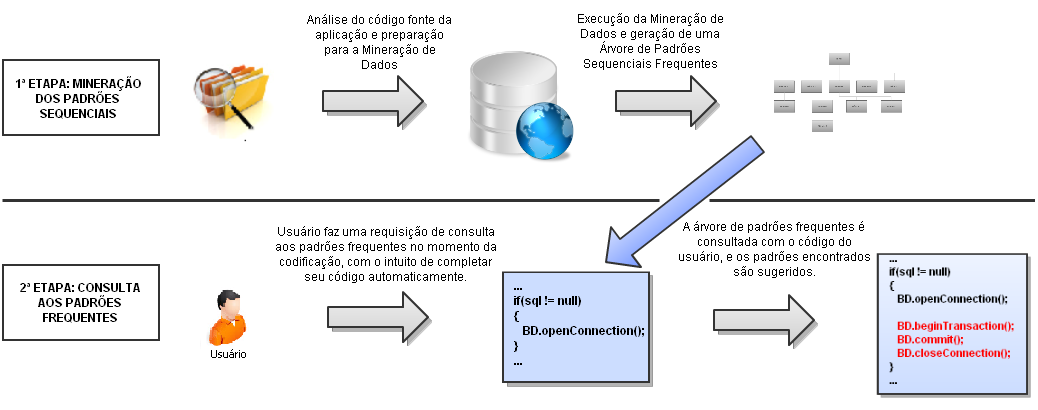
\includegraphics[width=1.0\textwidth]{fluxo.png}
			\FigLegenda{\label{fig:fluxo}Fluxo de uso do VCC.}
	\end{center}
\end{figure}

\section{Obten��o de Padr�es Frequentes de Codifica��o de Software.}

Esta se��o est� dividida em outras tr�s subse��es. O processo de an�lise de c�digo fonte � apresentado na Subse��o 3.1.1. Em seguida, a estrat�gia de minera��o de dados � descrita na Subse��o 3.1.2. Por �ltimo, a estrutura de armazenamento dos padr�es obtidos � detalhada na Subse��o 3.1.3.

\subsection{An�lise do C�digo Fonte}

Para que seja poss�vel, atrav�s de uma fonte de dados pr�-existente, sugerir padr�es frequentes de c�digo fonte, � necess�rio que os dados estejam coesos e estruturados para execu��o de consultas. Contudo, isso n�o � uma realidade inicial para o contexto desse trabalho, visto que o c�digo de uma aplica��o � armazenado em formato texto, sem obedecer a padr�es r�gidos de estrutura��o. Felizmente, cada linguagem de programa��o obedece a um conjunto de regras de formata��o, que s�o necess�rias para a compila��o adequada do c�digo fonte em linguagem de m�quina.

Dessa forma, embora n�o seja poss�vel fornecer diretamente arquivos de c�digo como entrada para minera��o sequencial de dados, os padr�es da linguagem de programa��o podem ser utilizados para se extrair as informa��es pertinentes do c�digo fonte e organiz�-las no formato de sequ�ncias de eventos. Conforme visto no Cap�tulo 2, atrav�s da an�lise de eventos que ocorrem em sequ�ncia, � poss�vel detectar padr�es frequentes que obedecem a uma determinada sequ�ncia. Todavia, em cada dom�nio de aplica��o, sequ�ncias, eventos e os itens que comp�em cada evento possuem significados distintos~\cite{LivroMineracao}.

 Neste trabalho, os eventos de uma sequ�ncia est�o todos em um mesmo corpo de m�todo, e cada evento � uma chamada de m�todo. Com isso, n�o � poss�vel dividir o evento em diferentes itens, sendo ent�o cada evento at�mico. Dessa forma, os padr�es sequenciais minerados s�o listas de chamadas de m�todo, que obedecem a uma determinada sequ�ncia e se repetem frequentemente em diferentes corpos de m�todos. � importante ressaltar que as estruturas de controle do c�digo fonte n�o s�o consideradas na obten��o das chamadas de m�todos, sendo cada corpo de m�todo uma �nica sequ�ncia de chamadas.

Na Figura \ref{fig:metodo-transacao}, � poss�vel visualizar a rela��o entre a codifica��o de um m�todo e sua respectiva sequ�ncia de eventos. 

%\begin{figure}
%	\begin{center}
%		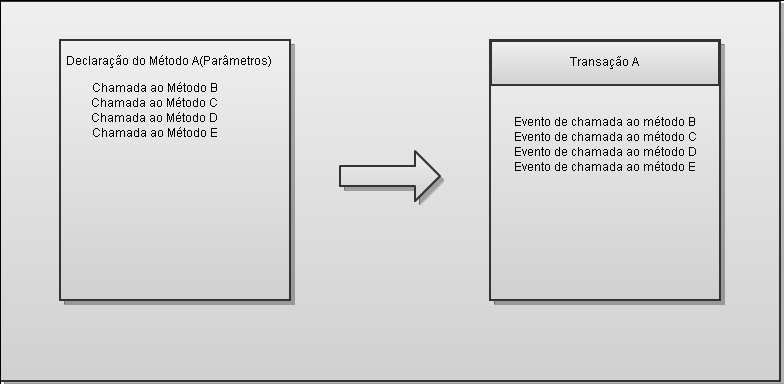
\includegraphics[width=0.85\textwidth]{metodo-transacao.png}
%			\FigLegenda{\label{fig:metodo-transacao}Exemplo de codifica��o de m�todo e a transa��o gerada.}
%	\end{center}
%\end{figure}

\begin{figure}[htb]
       \centering  % figura centralizada
       \fbox{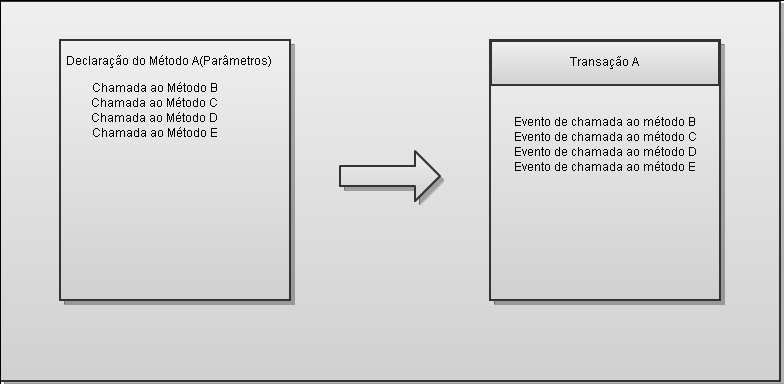
\includegraphics[scale=0.5]{metodo-transacao.png}}
       \FigLegenda{\label{fig:metodo-transacao}Exemplo de codifica��o de m�todo e a sequ�ncia gerada.}
       %\caption{\it Exemplo de codifica��o de m�todo e a transa��o gerada.}
       %\label{fig:metodo-transacao}
\end{figure}

\subsection{Minera��o do C�digo Fonte}

Existem diversos algoritmos para realizar minera��o de padr�es sequenciais, cada um com suas particularidades de entrada e sa�da. Organizando os dados de uma maneira que atenda a essas particularidades, a minera��o de padr�es sequenciais pode ent�o ser realizada, mas para que os resultados desse processo sejam proveitosos, dois conceitos s�o essenciais: suporte e confian�a.

O suporte j� foi definido anteriormente, no Cap�tulo 2, e sabe-se que � a quantidade de vezes que um determinado padr�o se repete na base de dados. Portanto, � poss�vel definir um suporte m�nimo para a obten��o desses padr�es, filtrando os padr�es mais frequentes. 

A confian�a, por outro lado, � muito importante nas regras de associa��o e representa uma m�trica de avalia��o que traz uma maior riqueza para a apresenta��o de regras mineradas. Entretanto, apesar de tradicionalmente n�o ser um conceito utilizado na minera��o de padr�es sequenciais, � definido e utilizado neste trabalho.

Para definir a confian�a em padr�es sequenciais, primeiramente � apresentada a defini��o de confian�a em regras de associa��o. Consequentemente, � necess�rio que tamb�m seja apresentada a defini��o do suporte de uma regra de associa��o.

O suporte de um conjunto de itens A, consiste na porcentagem de transa��es da base de dados que cont�m esse conjunto de itens, e pode ser representado por Sup(A). 

A confian�a pode ser definida em termos do suporte. Ou seja, dado uma regra de associa��o A $\rightarrow$ B, onde A e B s�o conjuntos de itens, a confian�a dessa regra representa a porcentagens de transa��es que cont�m B, dentre todas as transa��es que cont�m A, ou seja, Conf$\left(A \rightarrow B\right)$ = Sup$\left(A\cup B\right)$ / Sup$\left(A\right)$~\cite{Goncalves}. Dessa forma, o suporte de uma regra A $\rightarrow$ B, representado por Sup$\left(A \rightarrow B\right)$ e definido por Sup$\left(A\cup B\right)$, � equivalente � probabilidade conjunta de A e B, P(A$\cap$B), e confian�a � equivalente � probabilidade condicional de B dado que A ocorre, P(B$|$A).

%� poss�vel ent�o definir a confian�a em minera��o de padr�es sequenciais, enxergando-a como uma deriva��o da existente em %regras de associa��o. Uma sequ�ncia \textbf{s}, representada por uma lista de eventos $<e_{1}e_{2}e_{3}...e_{n}>$, onde %e$_{j}$, $1 \leq j \leq $n, � dito um evento ou elemento da sequ�ncia \textbf{s}, pode ser subsequ�ncia de outra sequ�ncia %\textbf{S}, representada por uma lista de eventos que obrigatoriamente cont�m todos os eventos da sequ�ncia \textbf{s}. Sendo %assim, nomeando \textbf{s} como \textbf{SubSeq} e \textbf{S} como \textbf{SuperSeq} a confian�a de \textbf{SuperSeq} � %calculada como:

� poss�vel ent�o definir a confian�a em minera��o de padr�es sequenciais, enxergando-a como uma deriva��o da existente em regras de associa��o. Dada uma sequ�ncia \textbf{s}, e outra sequ�ncia \textbf{S}, que � supersequ�ncia de \textbf{s}, a confian�a de \textbf{S} em rela��o a \textbf{s}, ser� a porcentagem de sequ�ncias que cont�m \textbf{S} dentre todas as que cont�m \textbf{s}. Tem-se ent�o:

               \textbf{Confian�a$_{\textbf{S/s}}$ = Sup(S) / Sup(s)}
               
Esse conceito pode ser exemplificado da seguinte maneira: dado que um padr�o sequencial X, formado por $\left\{A, B, C, D\right\}$, possui suporte de 28\% e que o padr�o sequencial Y, formado por $\left\{A, B\right\}$, possui suporte de 35\%. A confian�a de X em rela��o a Y � de 80\%.

Com isso, a seguinte afirma��o pode ser empregada pelo VCC: usu�rios que chamam os m�todos A e B em sequ�ncia, tamb�m chamam, com 80\% de confian�a, os m�todos C e D.

\subsection{Gera��o de �rvore de Chamadas}

Para que os padr�es obtidos na fase de minera��o sequencial possam ser utilizados na sugest�o de c�digo fonte, uma estrutura adequada deve ser empregada para o armazenamento e consulta dos mesmos.

	Neste trabalho, � utilizada uma �rvore de profundidade e largura vari�veis para armazenar os padr�es frequentes obtidos. A Figura \ref{fig:arvore-sem-suporte} ilustra a estrutura de uma �rvore de padr�es frequentes, onde � poss�vel visualizar cinco padr�es sequenciais distintos. S�o eles: $<A, B>$, $<C, D, E>$, $<C, D>$, $<C, E>$ e $<D, E>$.
	
\begin{figure}[htb]
       \centering  % figura centralizada
       \fbox{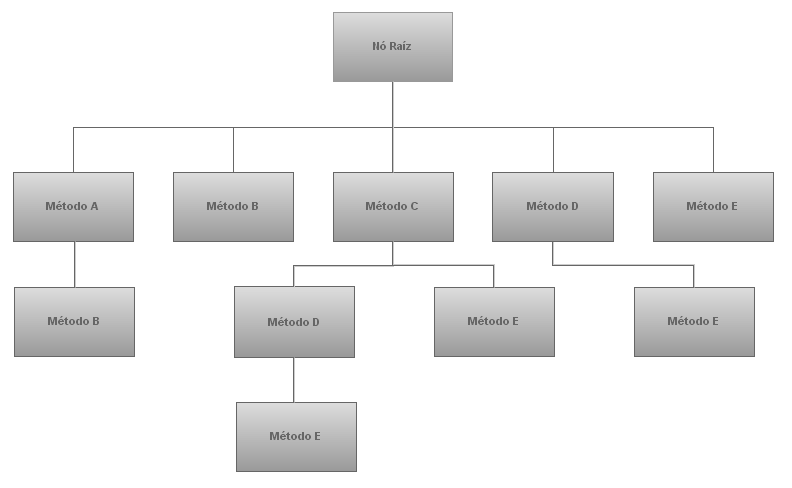
\includegraphics[scale=0.45]{arvore-sem-suporte.png}}
       \FigLegenda{\label{fig:arvore-sem-suporte}Exemplo de �rvore de padr�es frequentes.}
\end{figure}
	
	� importante ressaltar que a estrutura utilizada na cria��o da �rvore permite que a busca por uma sequ�ncia de c�digo tenha complexidade assint�tica~\cite{ProblemsAlgorithms} O$\left(n\right)$, sendo n o tamanho da sequ�ncia pesquisada. Isso acontece porque todos os elementos presentes na �rvore em n�veis mais profundos tamb�m est�o representados no segundo n�vel, conforme pode ser visto na Figura \ref{fig:arvore-sem-suporte} nos M�todos B, D e E.
	
	Apesar de parecer um desperd�cio proposital de espa�o de armazenamento para obter um melhor desempenho na busca por elementos da �rvore, a presen�a de todos os elementos frequentes no segundo n�vel da �rvore, se deve a um comportamento inerente � minera��o de padr�es sequenciais, que diz que se uma sequ�ncia � frequente, ou seja, possui suporte superior ao suporte m�nimo, todas as suas subsequ�ncias tamb�m ser�o frequentes. Isso pode ser observado na Figura \ref{fig:arvore-sem-suporte} nas ocorr�ncias do n� que representa o M�todo B, por exemplo. Embora esse m�todo j� esteja presente no terceiro n�vel da �rvore, representando a sequ�ncia $<A,B>$, � necess�rio que o mesmo tamb�m esteja presente no segundo n�vel representando padr�es sequenciais que possuam como primeiro evento frequente, justamente o M�todo B.  
	
	Ap�s definir a estrutura de armazenamento como uma �rvore, � importante que seja decidido o que cada n� ir� armazenar.  Considerando cada n� como o fim de um padr�o sequencial frequente, nos mesmos ser� armazenado o suporte desse padr�o. 
	
	Entretanto, a confian�a de um padr�o n�o pode ser vista como um �nico valor. A confian�a de um padr�o sequencial depende da subsequ�ncia que est� sendo consultada. Dessa forma, o tamanho do padr�o sequencial minerado determinar� quantos valores de confian�a o mesmo ter�. Dada uma sequ�ncia de tamanho igual a tr�s, X = $<C, D, E>$, as seguintes confian�as s�o definidas:

\begin{itemize}
	\item Confian�a de X em rela��o � sequ�ncia vazia. O valor dessa confian�a � o mesmo do suporte do padr�o sequencial; 
	\item Confian�a de X em rela��o � sequ�ncia $< C >$. O valor dessa confian�a ser� o suporte de X dividido pelo suporte de $< C >$;
	\item Confian�a de X em rela��o � sequ�ncia $< C, D >$. O valor dessa confian�a ser� o suporte de X dividido pelo suporte de $< C, D >$;
\end{itemize}

Dessa forma, uma gama de sugest�es pode ser fornecida ao usu�rio utilizador do VCC. Dado que uma chamada ao m�todo C, que possui suporte \textbf{s}, foi codificada, e que a sequ�ncia $< C, D >$, que est� presente na �rvore de padr�es sequenciais frequentes, possui suporte \textbf{S$_1$}, pode-se sugerir a chamada ao m�todo D, com confian�a \textbf{C$_1$}, dado que \textbf{C$_1$} = \textbf{S$_1$ / s}. Al�m disso, dado que a sequ�ncia $< C, D, E>$ tamb�m possui suporte \textbf{S$_2$}, superior ao suporte m�nimo, pode-se sugerir a sequ�ncia de chamadas $< D, E>$ com confian�a \textbf{C$_2$}, dado que \textbf{C$_2$} = \textbf{S$_2$ / s}.

A Figura \ref{fig:arvore} ilustra uma �rvore de padr�es sequenciais frequentes e a forma com que os suportes e confian�as s�o armazenados.

%\begin{figure}
%	\begin{center}
%		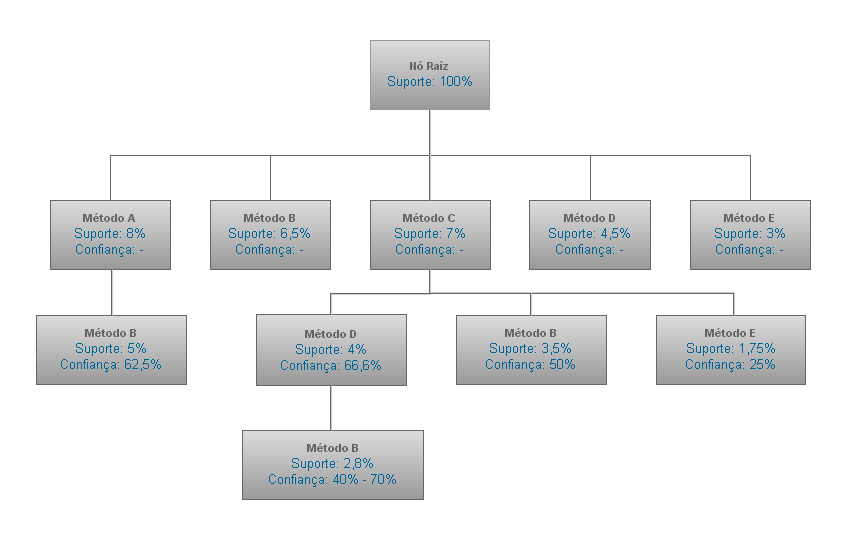
\includegraphics[width=1.0\textwidth]{arvore.png}
%			\FigLegenda{\label{fig:arvore}Exemplo de �rvore de padr�es frequentes com suportes e confian�as.}
%	\end{center}
%\end{figure}

\begin{figure}[htb]
       \centering  % figura centralizada
       \fbox{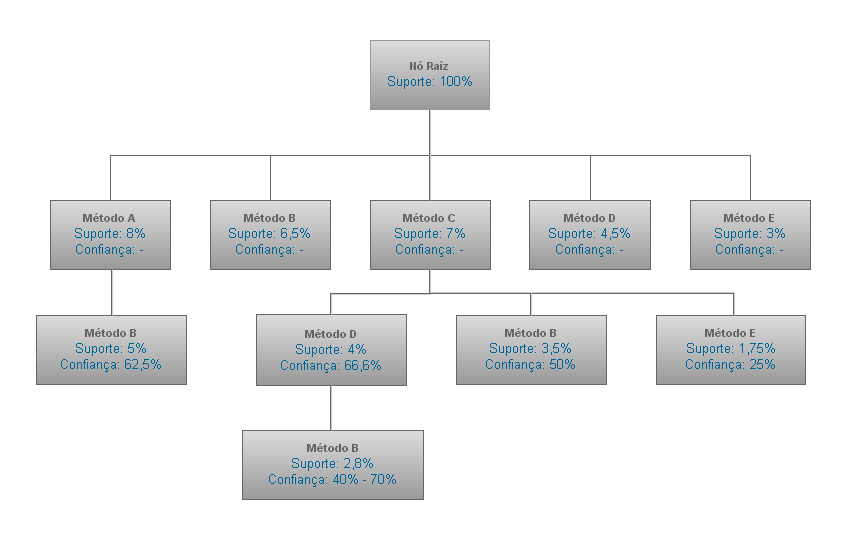
\includegraphics[scale=0.425]{arvore.png}}
       \FigLegenda{\label{fig:arvore}Exemplo de �rvore de padr�es frequentes com suportes e confian�as.}
\end{figure}


 Observando a sequ�ncia frequente $<C, D, E>$ por exemplo, as confian�as armazenadas no n� que representa o m�todo E, 40\% e 70\%, s�o respectivamente:

\begin{itemize}
	\item	A confian�a do padr�o sequencial $<C, D, E>$ com rela��o � sequ�ncia $<C>$ e 
	\item	A confian�a do padr�o sequencial $<C, D, E>$ com rela��o � sequ�ncia $<C, D>$.
\end{itemize}

\section{Sugest�o de Padr�es Frequentes de C�digo Fonte}

  Para que um padr�o sequencial possa ser sugerido, � necess�rio que uma entrada seja disponibilizada pelo usu�rio. Nesse momento, diversas estrat�gias podem ser tomadas para decidir como ser� feita a pesquisa do que est� sendo programado.

	Enquanto o projeto VCC estava sendo desenvolvido, algumas dessas estrat�gias foram testadas com o intuito de realizar poucas consultas, otimizando o tempo de resposta do programa. Utilizar apenas as �ltimas linhas que foram programadas, ou apenas combina��es de linhas cont�guas, mostrou-se infrut�fero, pois muitos padr�es interessantes passaram despercebidos por estarem dispostos de diversas maneiras no corpo do m�todo.
	
 Em um m�todo com dez linhas, por exemplo, um padr�o sequencial frequente pode ser detectado a partir de chamadas que est�o localizadas imediatamente uma ap�s a outra, como em chamadas que se encontram uma no in�cio e outra no fim do que j� foi programado. Um exemplo interessante de padr�es sequenciais que n�o se localizam contiguamente, s�o as aberturas e fechamentos de conex�es com bancos de dados. Ao abrir uma conex�o, espera-se que algum procedimento seja realizado na base de dados, antes que a mesma seja fechada.
 
 Com isso, fica expl�cita a necessidade de se intercalar de diferentes maneiras as chamadas de m�todo dispon�veis. Isso � feito atrav�s da combina��o das chamadas de m�todos, de todas as maneiras poss�veis. Todavia, muitas combina��es diferentes ainda poderiam ser geradas, fazendo com que o tempo de resposta para a consulta na �rvore de padr�es frequentes fosse longo. Isso porque mesmo sabendo que as boas pr�ticas de programa��o recomendam a filosofia de dividir para conquistar~\cite{Deitel}, m�todos em um projeto de software podem se tornar grandes demais.

Com isso, para que a consulta a todas as combina��es de chamadas de m�todos seja realizada em tempo h�bil, � necess�rio que o tamanho m�ximo dessas combina��es seja limitado. No VCC, o tamanho m�ximo das combina��es � configur�vel, permitindo que um valor que atenda �s caracter�sticas do projeto em quest�o seja alcan�ado. Entretanto, esse valor pode ser alto, gerando uma enorme quantidade de combina��es, e fazendo com que o tempo de resposta das consultas ainda n�o seja satisfat�rio.

Com o intuito de minimizar esse problema, a partir da an�lise das combina��es geradas, uma estrat�gia de poda foi desenvolvida, evitando que todas essas combina��es sejam consultadas. Essa estrat�gia parte do princ�pio de minera��o de padr�es sequenciais que garante que se uma sequ�ncia n�o � frequente, ent�o todas as supersequ�ncias dessa sequ�ncia tamb�m n�o s�o frequentes. No projeto VCC, a poda das sequ�ncias a serem consultadas na �rvore de padr�es acontece ap�s a consulta de uma sequ�ncia que n�o � frequente. Todas as outras sequ�ncias de m�todo que s�o supersequ�ncias desta s�o ent�o descartadas.

	Finalmente, ap�s todas as combina��es de chamadas de m�todos terem sido consultadas, os padr�es sequenciais obtidos s�o classificados de acordo com seus valores de suporte e confian�a e ent�o sugeridos para o usu�rio do VCC. O usu�rio pode ent�o analisar as sugest�es e escolher a que se ad�qua melhor ao que est� sendo desenvolvido.
	
	Utilizando como exemplo a �rvore da Figura \ref{fig:arvore}, pode-se supor que o usu�rio do VCC codifique chamadas aos m�todos A, D e F, e em seguida efetue uma requisi��o ao VCC, fazendo com que as seguintes combina��es de chamadas sejam geradas: $<A>$, $<D>$, $<F>$, $<A, D>$, $<A, F>$, $<D, F>$.
	
	Essas combina��es s�o ent�o consultadas na �rvore de padr�es frequentes, de acordo com o tamanho de cada combina��o. Ao consultar a chamada ao m�todo A, a chamada ao m�todo B seria obtida com suporte de 5\% e confian�a de 62,5\%. J� consultando a chamada ao m�todo D, a chamada ao m�todo E seria obtida com suporte de 3\% e confian�a de 66,6\%. Em seguida, ao consultar a chamada ao m�todo F nenhum padr�o seria encontrado, fazendo com que a poda de combina��es seja realizada. As combina��es $<A, F>$ e $<D, F>$ s�o ent�o 'podadas', evitando que sejam consultadas desnecessariamente.
  Finalmente, a combina��o $<A, D>$ � consultada na �rvore de padr�es frequentes e novamente nenhum padr�o � encontrado, como n�o existem outras combina��es a serem consultadas, a busca por padr�es se encerra, e os que foram encontrados s�o sugeridos ao usu�rio.
  � importante ressaltar que a combina��o $<A, D, F>$ n�o � nem mesmo gerada para ser consultada, visto que na �rvore n�o existe nenhum padr�o sequencial que possua mais de tr�s chamadas de m�todo.


\capitulo{Implementa��o}\label{cap:implementacao}

Cap�tulo 4


\capitulo{Resultados Experimentais}\label{cap:resultExperimentais}

Nesse cap�tulo s�o discutidos os resultados experimentais obtidos a partir da utiliza��o da abordagem proposta sobre o sistema objeto de estudo, o IdUFF - Sistema de Gest�o Acad�mica da Universidade Federal Fluminense. A se��o 5.1 apresenta o sistema utilizado no experimento. A se��o 5.2 apresenta o planejamento do experimento, seguido pela se��o 5.3, que aborda a aplica��o do experimento. Finalmente, as se��es 5.4 e 5.5 apresentam, respectivamente, os resultados obtidos e as amea�as � validade desse experimento.

\section{O sistema objeto de estudo - IdUFF}

O sistema IdUFF � o sistema de gest�o acad�mica utilizado na Universidade Federal Fluminense. Possui como principais funcionalidades a inscri��o on-line de alunos em disciplas, permitindo que aproximadamente 30 mil alunos escolham as disciplinas que v�o cursar no per�odo sem precisar comparecer a coordena��o do curso, como era feito antes do sistema existir, a gera��o de hist�ricos e comprovantes de regularidade de matr�cula on-line, al�m do m�dulo de lan�amento de notas pelos professores, entre outras. 

Ele foi escolhido para ser utilizado no experimento pela facilidade de contato com os desenvolvedores, que s�o ou foram alunos de gradua��o e p�s-gradua��o da UFF, e por ser um sistema de m�dio porte, que vem sendo desenvolvido h� 4 anos e apresenta uma grande quantidade de c�digo fonte a ser minerada. 

O mesmo foi desenvolvido sobre a plataforma Java, a mesma linguagem que o \textit{plugin} VCC foi desenvolvido para ser utilizado. Utiliza os frameworks Hibernate, que � respons�vel pelo mapeamento objeto/relacional da aplica��o Java, Spring que � respons�vel pela invers�o de controle e inje��o de depend�ncias no sistema e Mockito, respons�vel por simular o comportamento de certos objetos para realizar testes.
  
Possu� aproximadamente 40 mil usu�rios, entre alunos, professores e funcion�rios da Universidade.  O reposit�rio de c�digo fonte do IdUFF possui 4920 commits e o sistema IdUFF tem aproximandamente 850 revis�es. O sistema possui 779 classes Java, desconsiderando classes de teste, arquivos de interface HTML e arquivos de configura��o.


\section{Planejamento do Experimento}

Com o objetivo de avaliar o quanto as sugest�es de c�digo do \textit{plugin} VCC seriam �teis para um desenvolvedor que o estivesse utilizando, duas abordagens de experimento foram discutidas, ambas utilizando como base a experi�ncia de desenvolvimento do programador no sistema IdUFF. 

Na primeira abordagem, o pr�prio desenvolvedor utilizaria o \textit{plugin} VCC, instalado na sua IDE, ou seja, no seu ambiente de desenvolvimento do dia-a-dia de trabalho e, a partir disso, poderia avaliar se as sugest�es do \textit{plugin} seriam �teis. Por�m, esta abordagem n�o se mostrou interessante para ser aplicada nesse momento, pois al�m de demandar muito tempo, causaria muitos transtornos, pois o ambiente de desenvolvimento do sistema IdUFF utiliza uma IDE diferente da qual o \textit{plugin}  VCC foi acoplado. Outro ponto negativo dessa abordagem � que a usabilidade do \textit{plugin} n�o � o foco desse experimento, mas sim os resultados apresentados pelo mesmo.

Na segunda abordagem, uma an�lise em ambiente controlado poderia ser aplicada, obtendo-se padr�es de c�digo a partir da utiliza��o do \textit{plugin} VCC sobre o reposit�rio de c�digo fonte do sistema objeto de estudo e, a partir da�, construir um question�rio de avalia��o contendo alguns desses padr�es de c�digo pr�-selecionados.  Assim, cada volunt�rio poderia classificar, a partir de sua experi�ncia no desenvolvimento do sistema, se as sugest�es apresentadas fazem sentido ou n�o.

A segunda abordagem foi escolhida, justamente por permitir um maior controle sobre a avalia��o feita pelos desenvolvedores volunt�rios, garantindo-se que os mesmos padr�es fossem avaliados por todos. Assim, poder�amos avaliar se os resultados eram interessantes para os diversos perfis de desenvolvedores.

Para participar do experimento, os volunt�rios deveriam pertencer obrigatoriamente � equipe de desenvolvimento do sistema IdUFF. Seis desenvolvedores foram volunt�rios na participa��o desse experimento. N�o houve nenhum tipo de compensa��o para os participantes.



\section{Aplica��o do Experimento}

Inicialmente, cada volunt�rio foi informado do estudo atrav�s do Formul�rio de Consentimento (Ap�ndice I). Caso concordasse em participar, o Question�rio de Caracteriza��o (Ap�ndice II) era preenchido, avaliando o n�vel de conhecimento e experi�ncia do volunt�rio em diferentes temas relacionados ao estudo. Essas informa��es foram de grande utilidade, ajudando na interpreta��o dos resultados obtidos por cada um dos participantes.


A Tabela \ref{tab:resumo-caracterizacao} apresenta um resumo da caracteriza��o desses participantes. Os n�veis de experi�ncia variam de 0 a 4, onde 0 representa o n�vel mais baixo e 4 representa o n�vel mais alto de experi�ncia. 

\begin{table}
	\begin{center}
		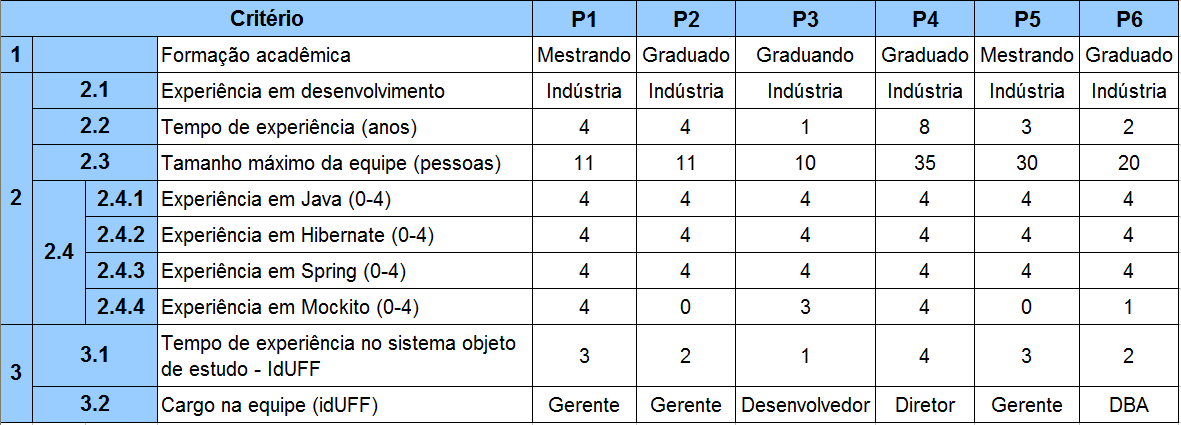
\includegraphics[width=1.0\textwidth]{resumo-caracterizacao.png}
		  \TabLegenda{\label{tab:resumo-caracterizacao}Resumo do Question�rio de Caracteriza��o dos participantes.}
			%\FigLegenda{\label{fig:resumo-caracterizacao}Resumo do Question�rio de Caracteriza��o dos participantes.}
	\end{center}
\end{table}


Na situa��o proposta aos participantes, um cen�rio fict�cio foi sugerido, onde os mesmos estariam programando uma linha de c�digo, por exemplo, chamando pelo m�todo \textit{br.uff.iduff2.mo\-delo.academico.Turma.getDisciplina()}, e o \textit{plugin} VCC iria exibir um padr�o, sugerindo que desenvolvedores que chamam esse m�todo tamb�m chamam o m�todo  \textit{br.uff.iduff2.modelo.aca\-demico.Disciplina.getCargaHorariaTeorica()}.

Assim, 10 padr�es de c�digo foram escolhidos, do total de 424 padr�es minerados atrav�s da utiliza��o do \textit{plugin} VCC, para serem analisados pelos desenvolvedores.  Esses padr�es foram obtidos utilizando-se um suporte m�nimo de 0,3\%, ap�s testes com diversos valores, por apresentar um n�mero razo�vel de sequ�ncias mineradas e ter um tempo de processamento relativamente r�pido, aproximadamente 15 segundos. O crit�rio de escolha dos 10 padr�es adotados foi buscar por padr�es de confian�a alta e confian�a baixa, o que permitiu uma avalia��o a partir dessas informa��es.

Os volunt�rios ent�o preencheram o Question�rio de Avalia��o (Ap�ndice III), por meio do qual expressavam sua opini�o com rela��o a cada sugest�o, podendo optar pelas seguintes respostas: n�o sei, discordo totalmente, discordo parcialmente, concordo parcialmente e concordo plenamente. As respostas foram dispostas exatamente nessa ordem de aceita��o da sugest�o. 


\section{Resultados Obtidos}

Como visto na se��o 5.3, 6 volunt�rios participaram do experimento, todos eles com experi�ncia em desenvolvimento de software. Os resultados obtidos do question�rio de avalia��o foram, em geral, positivos com rela��o � utilidade das sugest�es de c�digo informadas. Grande parte dos volunt�rios se mostrou interessada no \textit{plugin}, e gostaria de v�-lo sendo utilizado em seu ambiente de trabalho, se disponibilizando para ajudar a implementar as altera��es necess�rias para que o mesmo seja utilizado na IDE \textit{NetBeans}.


\subsection{An�lise Quantitativa}



Das 60 respostas obtidas a partir do preenchimento do question�rio de avalia��o pelos volunt�rios, 43 foram positivas, sendo 11 marcadas como \textit{concordo parcialmente} e 32 marcadas como \textit{concordo totalmente}, indicando assim um �ndice de 71,66\% de aceita��o das sugest�es de c�digo fonte. Foram 12 respostas negativas, sendo 6 marcadas como \textit{discordo totalmente} e 6 marcadas como \textit{discordo parcialmente}, indicando um �ndice de 20\% de reprova��o das sugest�es apresentadas. Do total das 60 respostas, 5 respostas foram marcadas como \textit{n�o sei}, sendo 8,33\% desse total. A figura \ref{fig:histograma} apresenta o total de respostas para cada item que poderia ser escolhido. A tabela \ref{tab:tab-questoes-suporte} apresenta um resumo detalhado das respostas, em porcentagem, de cada quest�o.


\begin{figure}[!htb]
	\begin{center}
		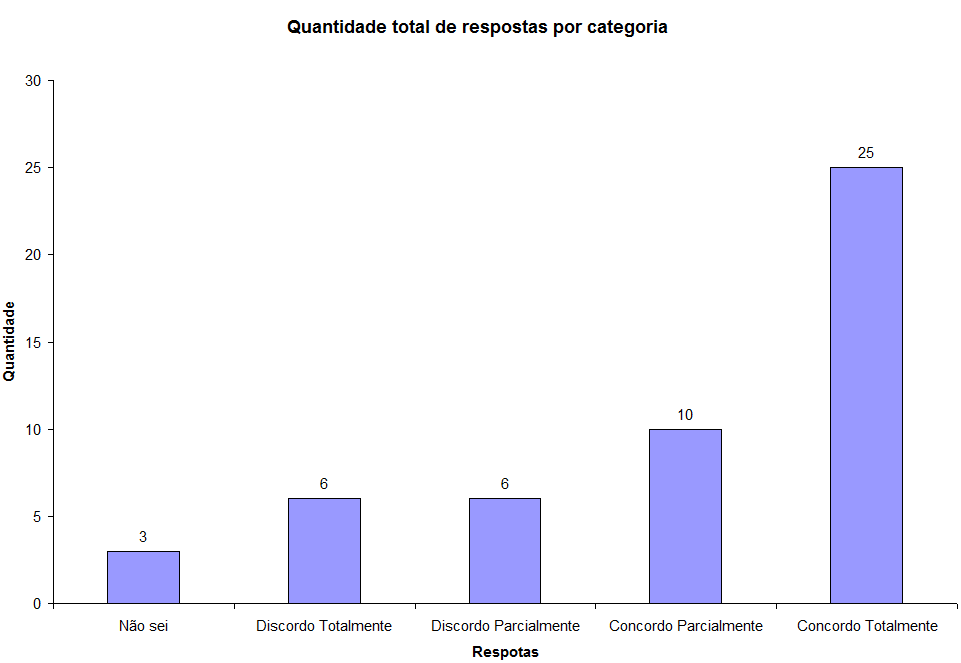
\includegraphics[width=1.0\textwidth]{histograma.png}
			\FigLegenda{\label{fig:histograma}Total de respostas dos participantes para cada item.}
	\end{center}
\end{figure}


\begin{table}[!htb]
	\begin{center}
		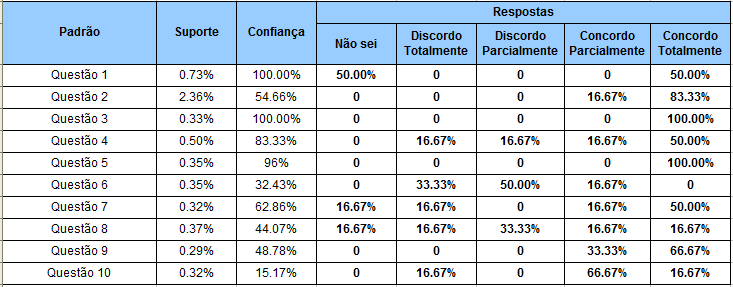
\includegraphics[width=1.0\textwidth]{tab-questoes-suporte.png}
		  \TabLegenda{\label{tab:tab-questoes-suporte}Resumo das respostas de cada quest�o, em porcentagem.}
			%\FigLegenda{\label{fig:resumo-caracterizacao}Resumo do Question�rio de Caracteriza��o dos participantes.}
	\end{center}
\end{table}

Foi feita tamb�m uma an�lise, relacionando a experi�ncia dos desenvolvedores volunt�rios e o valor de confian�a dos padr�es encontrados. Para essa an�lise, foram considerados 2 grupos de desenvolvedores: experientes, com 3 ou mais anos de experi�ncia no sistema IdUFF, e n�o experientes, com 2 anos ou menos de experi�ncia. Cada um dos grupos ficou com 3 desenvolvedores dentro desse perfil de experi�ncia. As sugest�es tamb�m foram separadass em 2 grupos: sugest�es com confian�a alta, com valores iguais ou superiores � 60\%, e sugest�es com confian�a baixa, com valores abaixo de 60\%.


\begin{figure}
	\begin{center}
		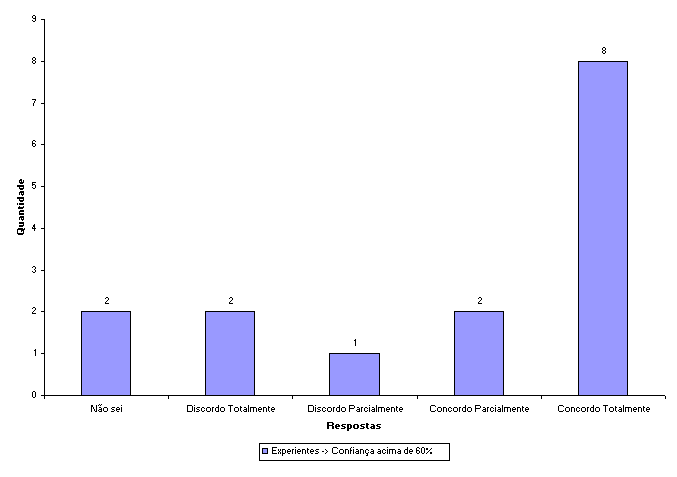
\includegraphics[width=0.9\textwidth]{hist-exp-conf-alta.png}
			\FigLegenda{\label{fig:hist-exp-conf-alta}Total de respostas, por item, dos participantes com experi�ncia alta nas quest�es com padr�es de confian�a alta.}
	\end{center}
\end{figure}

\begin{figure}
	\begin{center}
		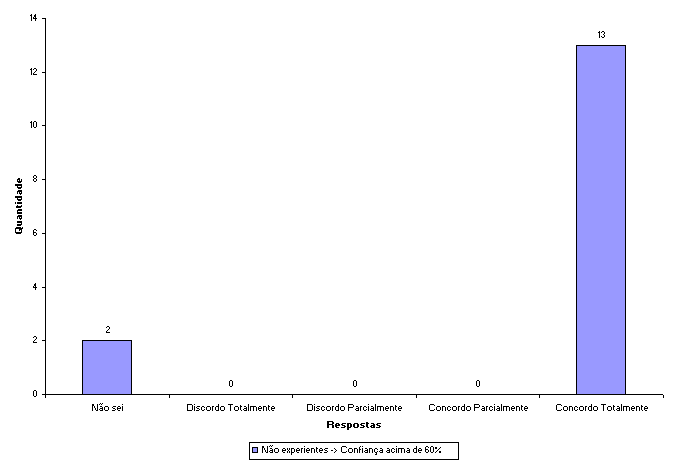
\includegraphics[width=0.9\textwidth]{hist-nao-exp-conf-alta.png}
			\FigLegenda{\label{fig:hist-nao-exp-conf-alta}Total de respostas, por item, dos participantes n�o experientes nas quest�es com padr�es de confian�a alta.}
	\end{center}
\end{figure}


\begin{figure}
	\begin{center}
		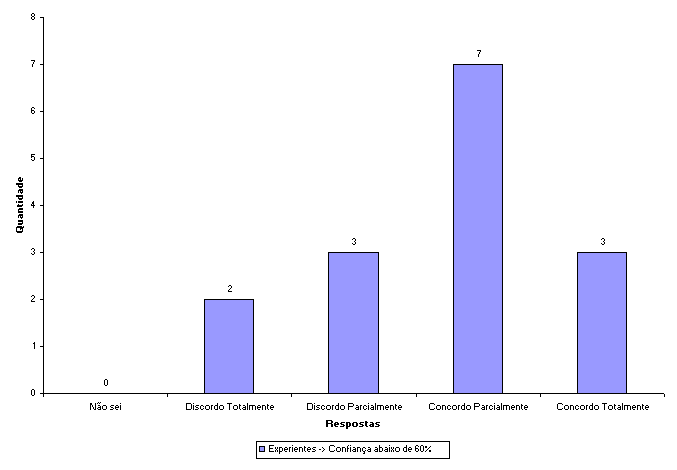
\includegraphics[width=0.9\textwidth]{hist-exp-conf-baixa.png}
			\FigLegenda{\label{fig:hist-exp-conf-baixa}Total de respostas, por item, dos participantes com experi�ncia alta nas quest�es com padr�es de confian�a baixa.}
	\end{center}
\end{figure}


\begin{figure}
	\begin{center}
		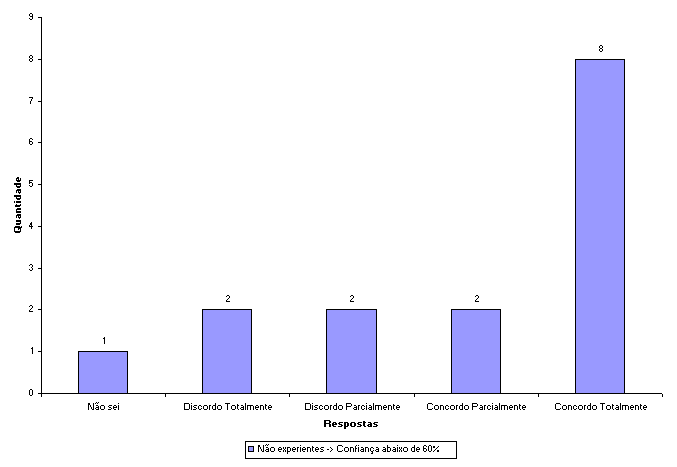
\includegraphics[width=0.9\textwidth]{hist-nao-exp-conf-baixa.png}
			\FigLegenda{\label{fig:hist-nao-exp-conf-baixa}Total de respostas, por item, dos participantes n�o experientes nas quest�es com padr�es de confian�a alta.}
	\end{center}
\end{figure}


Os gr�ficos das figuras \ref{fig:hist-exp-conf-alta}, \ref{fig:hist-nao-exp-conf-alta}, \ref{fig:hist-exp-conf-baixa} e \ref{fig:hist-nao-exp-conf-baixa} relacionam a experi�ncia dos desenvolvedores com a confian�a dos padr�es e permitem a visualiza��o do total de respostas dos volunt�rios para cada item. 




\subsection{An�lise Qualitativa}


Com rela��o as sugest�es com confian�a alta, os volunt�rios n�o experientes se mostraram muito satisfeitos, respondendo \textit{concordo plenamente} em 13 das 15 respostas que poderiam ser dadas para esse grupo de desenvolvedores. As outras 2 respostas foram marcadas como \textit{n�o sei}. J� os desenvolvedores experientes, responderam de forma positiva em 10 das 15 respostas poss�veis. A partir desses n�meros, fica claro que as sugest�es com confian�a alta tiveram um �ndice de aceita��o bom, tanto para os desenvolvedores experientes quanto para os n�o experientes.

As sugest�es com confian�a baixa, como esperado, foram as que mais receberam respostas negativas. Foram 5 respostas negativas dos desenvolvedores experientes e 4 dos n�o experientes, totalizando 9 dessas respostas. Com rela��o as respostas positivas, os desenvolvedores experientes foram os que mais fizeram ressalvas, marcando 7 sugest�es como \textit{concordo parcialmente} e 3 como \textit{concordo plenamente}. J� os desenvolvedores n�o experientes marcaram 2 sugest�es como \textit{concordo parcialmente} e 8 como \textit{concordo plenamente}. Esses n�meros mostram que, para os desenvolvedores experientes, as sugest�es com confian�a baixa se mostraram, em geral, �teis, por�m com a utiliza��o com alguma restri��o. 



As sugest�es 6 e 8 foram as que mais receberam respostas negativas, contabilizando 8 do total de 12 respostas nesse contexto. Dessas 8 sugest�es, 5 foram marcadas por desenvolvedores experientes. Esse resultado j� era esperado j� que essas sugest�es foram escolhidas por apresentarem confian�a baixa. Os volunt�rios que marcaram a sugest�o 6 negativamente, comentaram que a sugest�o apresentada n�o fazia sentido por n�o ser muito usada, e sugeriram outros padr�es de chamada de m�todo.

A sugest�o 10 recebeu a resposta \textit{discordo totalmente} por um dos volunt�rios e o coment�rio do mesmo foi pertinente � sugest�o apresentada: ``Se usa o m�todo \textit{BaseMB.info(String)} para mensagens que indiquem sucesso, n�o faz sentido exibir uma mensagem proveniente de uma situa��o de erro. Na minha opini�o, essa regra apresentada � aplic�vel aos m�todos \textit{BaseMB.er\-ror(String)} e \textit{BaseMB.warn(String)}''. Esse coment�rio reflete uma das limita��es desse projeto: n�o levar em conta blocos de repeti��o, condi��o e tratamento de erros, como no caso da estrutura \textit{try catch}. Geralmente o m�todo \textit{BaseMB.info(String)} � usado dentro de uma estrutura \textit{try}, e � executado se houver sucesso na opera��o, enquanto o m�todo \textit{java.lang.Throwable.getMessa\-ge()} � utilizado dentro de uma estrutura \textit{catch}, indicando um erro sendo lan�ado na aplica��o. Sendo assim, se a estrutura \textit{try catch} fosse levada em considera��o ao se buscar os padr�es sequ�ncias, essa sugest�o n�o seria minerada, j� que o m�todo \textit{java.lang.Throwable.getMessage()} n�o se enquadraria como uma sequ�ncia para o m�todo \textit{BaseMB.info(String)}.

A sugest�o 1 foi a que mais recebeu respostas \textit{n�o sei}, contabilizando 3 de um total de 5. Isso pode ser justificado pelo question�rio de caracteriza��o, onde os volunt�rios que responderam essa sugest�o dessa maneira s�o os que indicaram ter pouca ou nenhuma experi�ncia com o \textit{framework} de testes \textit{Mockito}. A sugest�o apresentada est� relacionada a esse \textit{framework}. As outras respostas obtidas para essa sugest�o foram bem satisfat�rias: 3 respostas \textit{concordo plenamente}. Essa sugest�o apresentava um suporte baixo, por�m uma confian�a alta, com valor de 100\%. Os desenvolvedores que comentaram essa sugest�o disseram que a sugest�o apresentada se d� por conta da estrutura do \textit{framework Mockito} e seria bastante �til sua utiliza��o.

As sugest�es que foram respondidas como \textit{concordo totalmente} e \textit{concordo parcialmente}, em geral n�o receberam coment�rios.



\section{Amea�as � Validade}


A sele��o dos participantes foi feita por meio da solicita��o de volunt�rios dentro da equipe de desenvolvimento do sistema IdUFF, a qual um dos pesquisadores faz parte como desenvolvedor. Como consequ�ncia, os resultados podem ter sido influenciados pela rela��o de amizade entre os volunt�rios e o pesquisador.  O pequeno n�mero de participantes e o tempo curto para aplica��o do experimento foi outro fator importante, pois � poss�vel que os resultados sejam influenciados pelo tamanho e pelas caracter�sticas espec�ficas do grupo.

A quantidade de sugest�es avaliadas pelos volunt�rios era pequena e simplificada, exibindo somente uma sugest�o onde poderiam ser sugeridas v�rias outras. Isso foi necess�rio devido a limita��o de tempo para o preenchimento do question�rio por meio dos volunt�rios e tamb�m para an�lise dos resultados.







\capitulo{Conclus�es}\label{cap:Conclusao}

  Nesse trabalho foi apresentada uma abordagem complementar a t�cnica de \textit{code completion}, o Vertical Code Completion que utiliza a Minera��o de Dados para extrair padr�es sequenciais frequentes e sugerir linhas de c�digo de fonte complementares, de acordo com o que j� foi programado. Assim, diferentemente do \textit{code completion}, que fornece ao desenvolvedor apenas sugest�es sint�ticas de c�digo fonte, o Vertical Code Completion traz sugest�es sem�nticas.

	Como contribui��o direta desse trabalho, foi desenvolvido um plugin que auxilia na produ��o de c�digo fonte, trazendo potenciais resultados positivos no desenvolvimento de software, como a exibi��o de conhecimento impl�cito ao c�digo. Isso p�de ser visto na utiliza��o do \textit{plugin} em um sistema real, o IdUFF. Os resultados obtidos nesse experimento foram positivos, indicando sucesso na abordagem proposta e na sua implementa��o, o \textit{plugin} VCC.
	
	O conceito de confian�a na minera��o de padr�es sequenciais frequentes foi outra contribui��o  apresentada nessa monografia. Esse conceito foi derivado da tarefa de regras de associa��o e sua defini��o � an�loga � dessa tarefa, fornecendo mais uma m�trica para avalia��o dos padr�es sequenciais obtidos.
	
 Contudo, algumas limita��es e trabalhos futuros foram identificados. A falta de um ambiente com um n�mero maior de desenvolvedores dispon�veis para responder ao question�rio de sugest�es da ferramenta, desfavoreceu a confiabilidade do experimento, tornando-se uma limita��o nessa monografia.
Al�m disso, um poss�vel trabalho futuro, que pode aumentar a qualidade das sugest�es produzidas pelo VCC, � a an�lise do c�digo fonte levando em considera��o as estruturas de repeti��o e principalmente de condi��o. Com isso, uma estrutura condicional, que possui mais de uma alternativa, n�o seria vista como uma �nica sequ�ncia de chamadas, e sim como sequ�ncias independentes. Al�m disso, outra poss�vel melhoria, com o intuito de aumentar a usabilidade da ferramenta, � o preenchimento autom�tico do c�digo fonte no editor da IDE em resposta � uma sugest�o aceita, ao inv�s de exibir as sugest�es em uma janela \textit{popup}.

% Cap�tulo de conclus�o
%\input{conclusao}

% Bibliografia
\nocite*

\bibliographystyle{plain-br}

%ler bibliografia.bib
\bibliography{bibliografia}

% In�cio dos ap�ndices
%\apendices

% Inclus�o do primeiro ap�ndice
\appendix
\addcontentsline{toc}{chapter}{AP�NDICE I}
\appendix{AP�NDICE I}\label{ape:apendice1}

\begin{center} {\Large Formul�rio de Consentimento}
\end{center}

\noindent \textbf{Estudo}

Este estudo visa avaliar o quanto as sugest�es de c�digos, informadas atrav�s do plugin Vertical Code Completion (VCC), s�o consistentes e fazem sentido no desenvolvimento, tanto para um desenvolvedor experiente quanto para um desenvolvedor novo na equipe.

\noindent \textbf{Idade}

Eu declaro ter mais de 18 anos de idade e concordar em participar de um estudo conduzido por Thiago Nazareth de Oliveira e Luiz Laerte Nunes da Silva Junior na Universidade Federal Fluminense.

\noindent \textbf{Procedimento}

Este estudo acontecer� em uma �nica sess�o, que incluir� a an�lise de algumas sugest�es de c�digo, retiradas do sistema IdUFF atrav�s do plugin VCC. Eu entendo que, uma vez o experimento tenha terminado, os trabalhos que desenvolvi ser�o estudados visando entender a efici�ncia dos procedimentos e as t�cnicas propostas.

\noindent \textbf{Confidencialidade}

Toda informa��o coletada neste estudo � confidencial, e meu nome n�o ser� divulgado. Da mesma forma, me comprometo a n�o comunicar os meus resultados enquanto n�o terminar o estudo, bem como manter sigilo das t�cnicas e documentos apresentados e que fazem parte do experimento.

\noindent \textbf{Benef�cios e liberdade de desist�ncia}

Eu entendo que os benef�cios que receberei deste estudo s�o limitados ao aprendizado do material que � distribu�do e apresentado. Eu entendo que sou livre para realizar perguntas a qualquer momento ou solicitar que qualquer informa��o relacionada � minha pessoa n�o seja inclu�da no estudo. Eu entendo que participo de livre e espont�nea vontade com o �nico intuito de contribuir para o avan�o e desenvolvimento de t�cnicas e processos para a Engenharia de Software.

\bigskip 

\noindent \textbf{Pesquisadores respons�veis}

\noindent Thiago Nazareth de Oliveira\\
\noindent Instituto de Computa��o - Universidade Federal Fluminense (UFF)

\noindent Luiz Laerte Nunes da Silva Junior\\
\noindent Instituto de Computa��o - Universidade Federal Fluminense (UFF)

\bigskip 

\noindent \textbf{Professores respons�veis}

\noindent Prof. Leonardo Paulino Gresta Murta\\
\noindent Instituto de Computa��o - Universidade Federal Fluminense (UFF)

\noindent Prof. Alexandre Plastino\\
\noindent Instituto de Computa��o - Universidade Federal Fluminense (UFF)

\bigskip 

\noindent \textbf{Nome (em letra de forma):} \hrulefill 

\noindent \textbf{Assinatura: \rule{10cm}{.1mm}}   \textbf{Data: \hrulefill  }



\newpage
\addcontentsline{toc}{chapter}{AP�NDICE II}
\appendix{AP�NDICE II}\label{ape:apendice2}

\begin{center} {\Large Question�rio de Caracteriza��o}
\end{center}


\noindent Este formul�rio cont�m algumas perguntas sobre sua experi�ncia acad�mica e profissional.

\noindent \textbf{1) Forma��o Acad�mica}


\noindent( ) Doutorado\\
\noindent( ) Doutorando\\
\noindent( ) Mestrado\\
\noindent( ) Mestrando\\
\noindent( ) Gradua��o\\
\noindent( ) Graduando\\


\noindent Ano de ingresso: \rule{2cm}{.1mm}  Ano de conclus�o (ou previs�o de conclus�o): \rule{2cm}{.1mm}

\bigskip 

\noindent \textbf{2) Forma��o Geral}

\bigskip 

2.1) Qual � sua experi�ncia com desenvolvimento de software? (marque aqueles itens que melhor se aplicam)

\noindent( ) Nunca desenvolvi software.\\
\noindent( ) J� li material sobre desenvolvimento de software.\\
\noindent( ) J� participei de um curso sobre desenvolvimento de software.\\
\noindent( ) Tenho desenvolvido software para uso pr�prio.\\
\noindent( ) Tenho desenvolvido software como parte de uma equipe, relacionado a um curso.\\
\noindent( ) Tenho desenvolvido software como parte de uma equipe, na ind�stria.\\


\bigskip 

2.2) Por favor, explique sua resposta. Inclua o n�mero de semestres ou n�mero de anos de experi�ncia relevante em desenvolvimento de software. (E.g. ``Eu trabalhei por 2 anos como programador de software na ind�stria'')

\noindent \hrulefill\\
\noindent \hrulefill\\
\noindent \hrulefill\\

\bigskip 

2.3) Qual � sua experi�ncia com desenvolvimento de software em equipes? Qual a
maior equipe de que voc� participou?

\noindent \hrulefill\\
\noindent \hrulefill\\

\bigskip

2.4) Por favor, indique o grau de sua experi�ncia nesta se��o seguindo a escala de 5 pontos abaixo:

\noindent 0 = nenhum\\
\noindent 1 = estudei em aula ou em livro\\
\noindent 2 = pratiquei em projetos em sala de aula\\
\noindent 3 = usei em projetos pessoais\\
\noindent 4 = usei em projetos na ind�stria\\

\bigskip

2.4.1) Linguagem JAVA\\
Respota:  \rule{2cm}{.1mm}

\bigskip

2.4.2) Hibernate\\
Resposta: \rule{2cm}{.1mm}

\bigskip

2.4.3) Spring\\ 
Resposta: \rule{2cm}{.1mm}

\bigskip

2.4.4) Mockito\\
Respota: \rule{2cm}{.1mm}

\bigskip

\noindent \textbf{3) Experi�ncia no desenvolvimento do sistema objeto de estudo - IdUFF} 

\bigskip

3.1) H� quanto tempo voc� est� na equipe de desenvolvimento do sistema IDUFF?\\
Resposta: \hrulefill

3.2) Qual o seu cargo na equipe? 

Resposta: \hrulefill
%\addcontentsline{toc}{chapter}{AP�NDICE I}
\appendix{AP�NDICE I}\label{ape:apendice1}

\begin{center} {\Large Formul�rio de Consentimento}
\end{center}

\noindent \textbf{Estudo}

Este estudo visa avaliar o quanto as sugest�es de c�digos, informadas atrav�s do plugin Vertical Code Completion (VCC), s�o consistentes e fazem sentido no desenvolvimento, tanto para um desenvolvedor experiente quanto para um desenvolvedor novo na equipe.

\noindent \textbf{Idade}

Eu declaro ter mais de 18 anos de idade e concordar em participar de um estudo conduzido por Thiago Nazareth de Oliveira e Luiz Laerte Nunes da Silva Junior na Universidade Federal Fluminense.

\noindent \textbf{Procedimento}

Este estudo acontecer� em uma �nica sess�o, que incluir� a an�lise de algumas sugest�es de c�digo, retiradas do sistema IdUFF atrav�s do plugin VCC. Eu entendo que, uma vez o experimento tenha terminado, os trabalhos que desenvolvi ser�o estudados visando entender a efici�ncia dos procedimentos e as t�cnicas propostas.

\noindent \textbf{Confidencialidade}

Toda informa��o coletada neste estudo � confidencial, e meu nome n�o ser� divulgado. Da mesma forma, me comprometo a n�o comunicar os meus resultados enquanto n�o terminar o estudo, bem como manter sigilo das t�cnicas e documentos apresentados e que fazem parte do experimento.

\noindent \textbf{Benef�cios e liberdade de desist�ncia}

Eu entendo que os benef�cios que receberei deste estudo s�o limitados ao aprendizado do material que � distribu�do e apresentado. Eu entendo que sou livre para realizar perguntas a qualquer momento ou solicitar que qualquer informa��o relacionada � minha pessoa n�o seja inclu�da no estudo. Eu entendo que participo de livre e espont�nea vontade com o �nico intuito de contribuir para o avan�o e desenvolvimento de t�cnicas e processos para a Engenharia de Software.

\bigskip 

\noindent \textbf{Pesquisadores respons�veis}

\noindent Thiago Nazareth de Oliveira\\
\noindent Instituto de Computa��o - Universidade Federal Fluminense (UFF)

\noindent Luiz Laerte Nunes da Silva Junior\\
\noindent Instituto de Computa��o - Universidade Federal Fluminense (UFF)

\bigskip 

\noindent \textbf{Professores respons�veis}

\noindent Prof. Leonardo Paulino Gresta Murta\\
\noindent Instituto de Computa��o - Universidade Federal Fluminense (UFF)

\noindent Prof. Alexandre Plastino\\
\noindent Instituto de Computa��o - Universidade Federal Fluminense (UFF)

\bigskip 

\noindent \textbf{Nome (em letra de forma):} \hrulefill 

\noindent \textbf{Assinatura: \rule{10cm}{.1mm}}   \textbf{Data: \hrulefill  }




\end{document}
